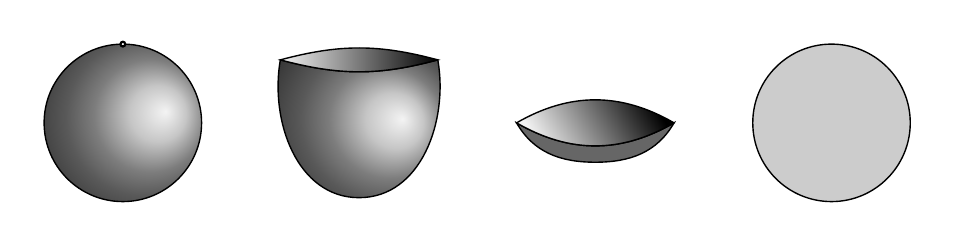
\begin{tikzpicture}[%
    line width=0.5pt,
    sphereshade/.style={
        ball color=gray!60!white,
        draw=black,
        shading angle=240
    }
]
    % Some space to prevent clipping the image in the PDF.
    \draw[draw=white] (-5.2, -1.2) rectangle (6.2, 1.2);

    % Points for the Second Blob.
    \coordinate (a) at (-1.0, -0.95);
    \coordinate (b) at (-2.0,  0.80);
    \coordinate (c) at ( 0.0,  0.80);

    % Points for the Third Blob.
    \coordinate (d) at (2.0, -0.5);
    \coordinate (e) at (1.0,  0.0);
    \coordinate (f) at (3.0,  0.0);

    % First blob (Sphere).
    \filldraw[sphereshade] (-4,0) circle (1);

    % North pole of the sphere is missing.
    \filldraw[white, draw=black, thick] (-4,1) circle (0.3mm);

    % Draw the second blob
    \draw[sphereshade] (a) to [out=180,in=-100] (b)
                           to [out=-15,in=-165] (c)
                           to [out=-80,in=0] cycle;

    \draw[left color=white!90!gray,right color=black]
        (b) to [out=-15,in=-165] (c)
            to [out=165,in=15] cycle;

    % Draw the third blob
    \draw[fill=black!20!gray] (d) to [out=180,in=-60] (e)
                                  to [out=-30,in=-150] (f)
                                  to [out=-120,in=0] cycle;

    \draw[left color=black, right color=white!90!gray,shading angle=300]
        (e) to [out=-30,in=-150] (f)
            to [out=150,in=30] cycle;

    % Draw the fourth blob (Circle)
    \filldraw[draw=black, fill=white!60!gray] (5,0) circle (1);
\end{tikzpicture}